The sinking slab benchmark consists of a beam of elastic material which is placed 
in a weak and viscous surrounding medium. The initially unstressed beam is attached 
to the left domain boundary through boundary conditions. A stress is then applied to 
the beam in the form of gravity. The applied gravity force results in the deformation 
of the beam through bending. After 20 kyr, the gravity field is turned off and the 
elastic properties of the beam will then force itself to its original position.  

\begin{center}
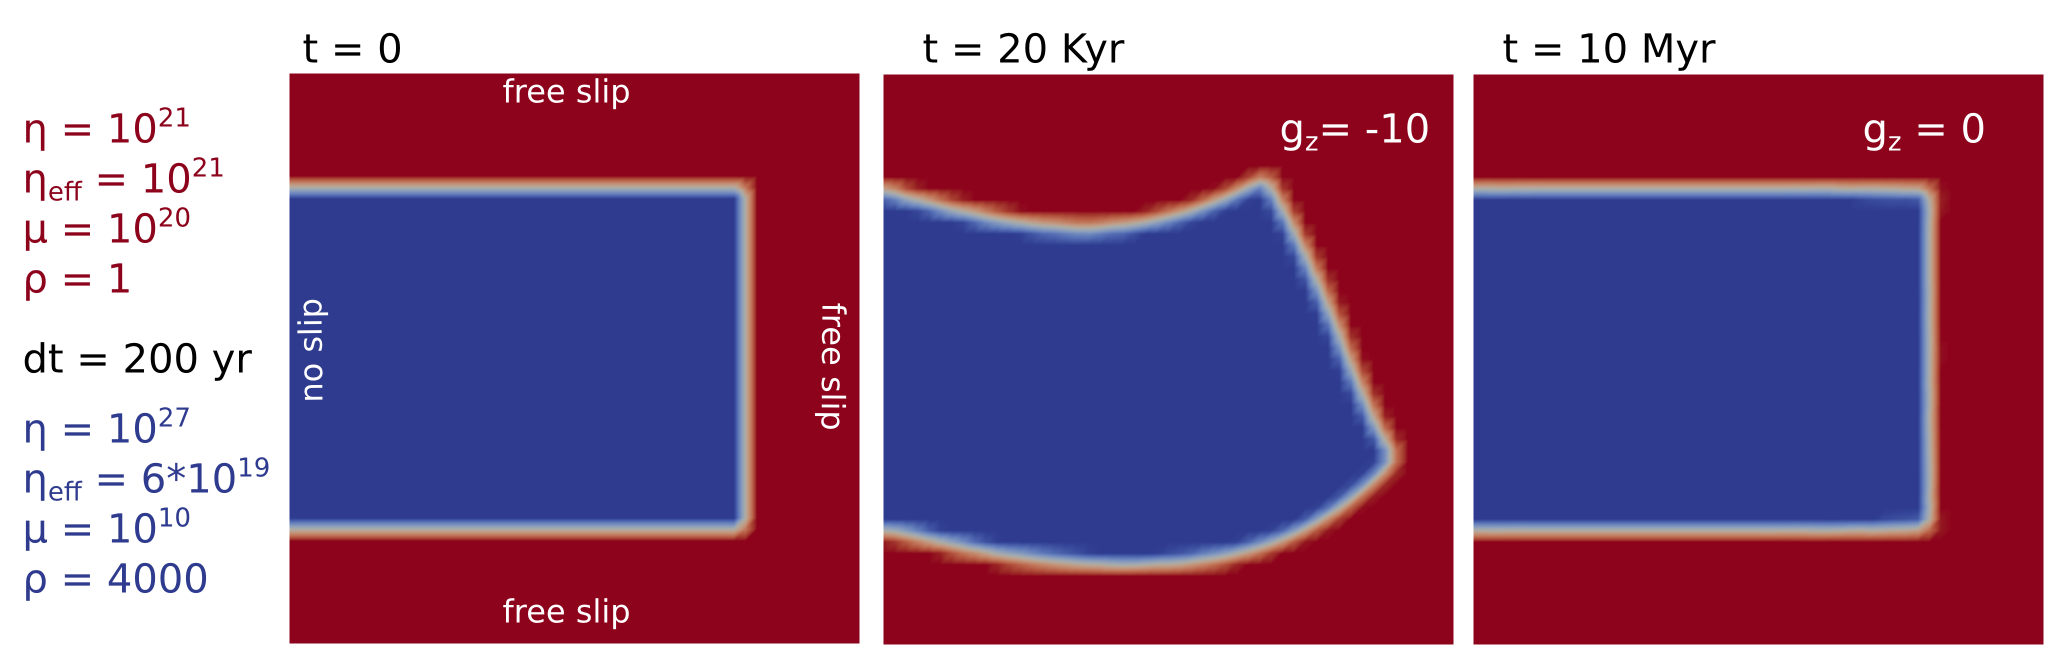
\includegraphics[width=0.9\textwidth]{python_codes/fieldstone_64/images/poster_benchmark.png}\\
\captionfont{Set-up and evolution of the benchmark from \cite{gery10}. The properties of the two materials are given on the left, together with the initial configuration of the benchmark. The middle panel shows the position of the beam at $t=20\ kyr$, the moment the gravity is set to zero. The right panel shows the end result of the beam after a recovery period of $9980\ kyr$ during the absence of gravity.   }
\end{center}


The set-up of the benchmark is given in the figure above. 
The beam is surrounded by a low-density, low-viscosity and high shear modulus medium 
of which the specifications are given in  the following table and the Figure. 
The boundary conditions of the domain consist of a no slip condition at 
the left boundary where the slab is attached and free slip boundary conditions along all other sides. 
The results are calculated on a grid with a resolution of 51 by 51 nodal points 
and 25 markers per element. 
The resolution and Courant number will be varied when using compositional fields to see 
if the models perform better with a higher resolution/lower time step. 

\begin{center}
\begin{tabular}{lll}
\textit{Material properties}& \textit{Elastic slab}  & \textit{Surrounding medium} \\ 
Density         $\rho$ \     [kg/m$^{3}$]      & 4000                    & 1     \\
Viscosity       $\eta$ \    [Pa$\cdot$ s]      & $10^{27}$                   &   $10^{21}$     \\
Shear modulus   $\mu $ \    [Pa]            & $10^{10}$                    & $10^{20}$       \\ 
\end{tabular} 
\end{center}

I have a nodal field for the two compositions, 1 is slab, 2 is mantle. 

$Delta t = 200yr$



